\documentclass[titlepage]{article}
\usepackage{listings}
\lstMakeShortInline{|}
\usepackage{courier}
\usepackage[colorlinks,linkcolor=blue,citecolor=blue,urlcolor=blue,breaklinks=true]{hyperref}
\lstset{basicstyle=\ttfamily\small , breaklines}
\usepackage[left=3cm,top=3cm,bottom=3cm, right=3cm,includehead,includefoot]{geometry}
\usepackage{fancyhdr,lastpage}
\pagestyle{fancy}
\rhead{Metrum Research Group LLC \\ }
\lhead{
\includegraphics[scale=.5]{logo.png}}
\cfoot{Page \thepage\ of \pageref{LastPage}}
\fancyhfoffset{.25in}
\renewcommand{\headrulewidth}{0.25pt}
\renewcommand{\footrulewidth}{0pt} 
\setlength{\headheight}{23pt}
\renewcommand{\labelitemiii}{$\circ$}
\usepackage{longtable}
\usepackage{amsmath}
\usepackage[T1]{fontenc}
\usepackage[scaled]{helvet}
\renewcommand*\familydefault{\sfdefault}
\usepackage{courier}
\usepackage{graphicx}
\usepackage{tocbibind}
\usepackage[parfill]{parskip}    % Activate to begin paragraphs with an empty line rather than an indent
\usepackage{upgreek}
\usepackage{textpos}
\usepackage{relsize}
\usepackage{upquote}
% Use \begin{landscape} and end{landscape} to rotate text %%%
\usepackage{pdflscape}
\usepackage{textcomp}
\usepackage{float}
\floatplacement{figure}{H}
\floatplacement{table}{H}
\usepackage[printonlyused,nohyperlinks]{acronym}
\def\bflabel#1{{\large#1\ \ \ \ }\hfill}
\usepackage{fixltx2e}
\setlength{\belowcaptionskip}{10pt}
\usepackage{Sweave}

 
\begin{document}
\vspace*{2cm}
\begin{center}
\vspace{1.5cm}
{\Large Wikimath}\\
~\\
\today\\
~\\
Tim Bergsma\\
\end{center}
\newpage

\section*{Wikimath}
\subsection{writing wikimath expressions}
Here we define a string of text.
\begin{Schunk}
\begin{Sinput}
> x <- "V_c /F (L * h^-1 ) ~theta_1 *(WT/70)^theta_2"
\end{Sinput}
\end{Schunk}
\subsection{extracting and supressing elements}
Now we try x as a column name for a data frame.
\begin{Schunk}
\begin{Sinput}
> d <- data.frame(subject=1,x=2)
> names(d)[2] <- wiki2label(x)
> d
\end{Sinput}
\begin{Soutput}
  subject V_c/F
1       1     2
\end{Soutput}
\begin{Sinput}
> justUnits(x)
\end{Sinput}
\begin{Soutput}
[1] "L * h^-1 "
\end{Soutput}
\end{Schunk}
\subsection{identifying related parameters}
What theta is primarily associated with this equation?
\begin{Schunk}
\begin{Sinput}
> wiki2parameter(x)
\end{Sinput}
\begin{Soutput}
[1] "THETA1"
\end{Soutput}
\begin{Sinput}
> text2decimal(wiki2parameter(x))
\end{Sinput}
\begin{Soutput}
[1] 1
\end{Soutput}
\end{Schunk}
\subsection{rendering in a table}
Next we try it in a latex table.
\begin{Schunk}
\begin{Sinput}
> writeLines(tabular(data.frame(model=wiki2latex(noUnits(x)))))
\end{Sinput}
\begin{tabular}{l}
  \hline \hline
 model \\ \hline
 $\mathrm{V_{c}/F  \sim\theta_{1}\cdot(WT/70)^{\theta_{2}}}$ \\ \hline
\end{tabular}\end{Schunk}
\subsection{rendering in a figure}
Finally we try it in a figure.
\begin{Schunk}
\begin{Sinput}
> library(lattice)
> print(densityplot(
+   ~v,
+   data.frame(v=rnorm(1000,mean=1)),
+   main=parse(text=wiki2plotmath(noUnits(x))),
+   xlab='volume (l)'
+ ))
\end{Sinput}
\end{Schunk}
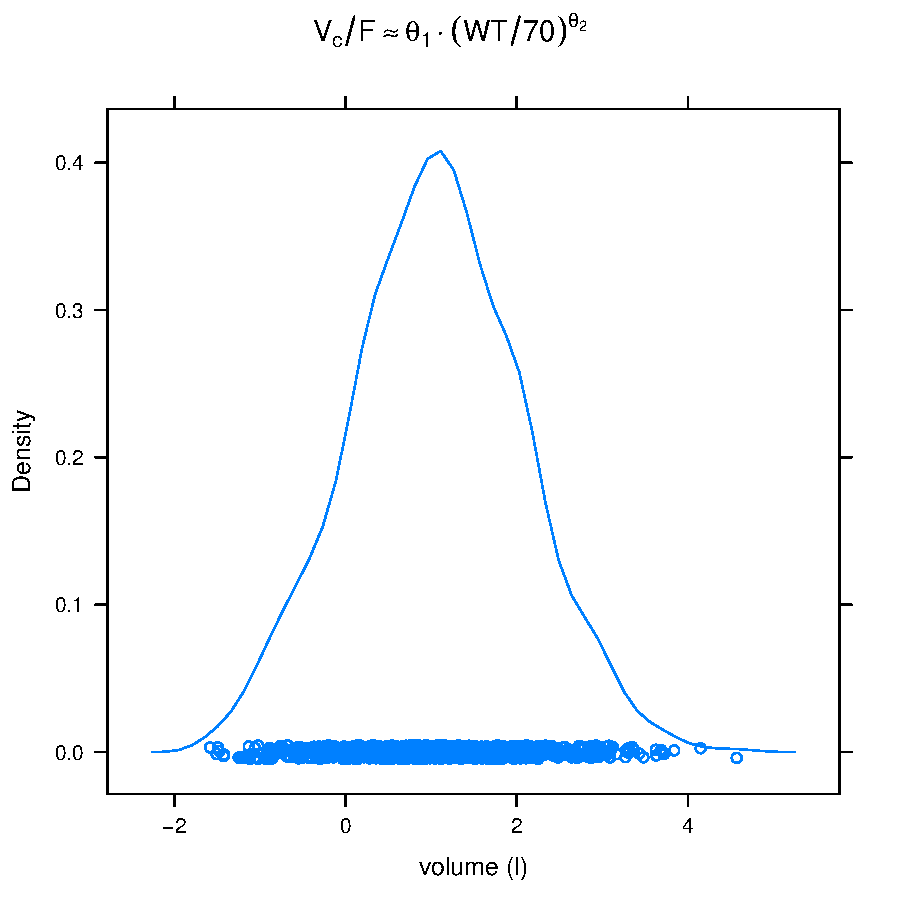
\includegraphics{wikimath-figure}
\end{document}
